%
% loesung.tex -- Beispiel-File für die Beschreibung der Loesung
%
% (c) 2020 Prof Dr Andreas Müller, Hochschule Rapperswil
%
\section{Lösung
\label{fem:section:loesung}}
\rhead{Lösung}
Wie im vorherigen Kapitel erwähnt, sind Herausforderungen bzw. Ansprüche an die Ansatzfunktionen zu beachten. Nun stellt sich die Frage, wie die Ansatzfunktion gewählt werden müssen, so das entlang eines Randes nur \frqq Knicke \flqq entstehen und keine Sprünge. Und wie ist gewährleistet das in jeder Stützstelle alle Elemente den gleichen Wert haben?  Als Lösungs bietet sich ein lineare Funktion an. Für ein Dreieck kann der Term $u(x) = c_1 + c_2x + c_3y$ verwendet werden. Diese Zusammensetzung ergibt sich, da der lineare Ansatz durch die Funktionswerte in den Ecken des Dreiecks bestimmt wird. In anderen Worten ausgedrückt sind die Funktionswerte in den Ecken des Teilgebiets, hier im Dreieck, die Unbekannten, die bestimmt werden müssen. Wie diese Koeffizienten in einer Matrix bestimmt werden ist in \ref{fem:section:GL} aufgezeigt.

%\begin{figure}[h!]
%	\centering
%	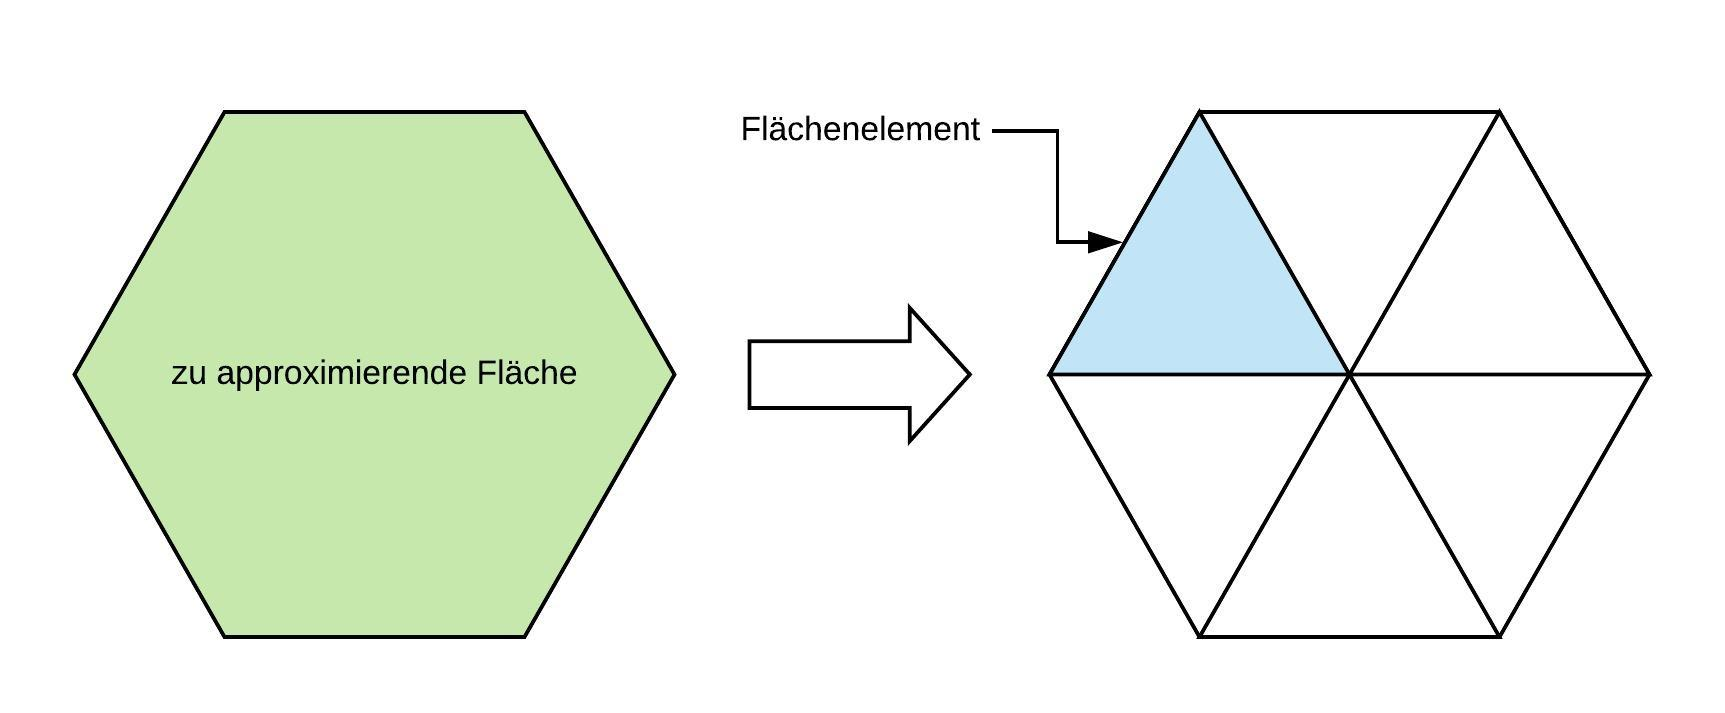
\includegraphics[scale=0.8]{papers/fem/Images/Approx.jpeg}
%	\caption{Flächen- Approximation mit Dreiecks- Flächenelemente}
%	\label{fem:Approx}
%\end{figure}
Nochmals zur Verdeutlichung warum ein linearer Ansatzfunktion verwendet wird:
\begin{itemize}
	\item eine einfache Formel gibt es nur auf einem kleinen Teilgebiet
	\item in dem Teilgebiet ist die Integral- Formel sehr einfach zu berechnen wie z.B. eine lineare Funktion die durch Koeffizienten bestimmt wird.
\end{itemize}
%ls Standardverfahren in der Ebene haben sich Flächenelement wie Dreiecken oder Parallelogramme bewährt. Die Wahl der  der Flächen- bzw. Gebiet- Elementen sollte so erfolgen, dass diese die zu approximierende Fläche möglichst gut nachbildet bzw. approxmimiert wird.
Um möglichst einfach darzustellen, wie das Verfahren der finiten Elemente vonstatten geht, wurde auf eine einfache Approximation mit Einheitsdreiecken und einem linearen Ansatz gewählt. 

\subsection{Vorbereitung
\label{fem:section:loesungTrans}}

Damit die Integration über das gewählte Teilgebiet einfacher fällt, wird als Vorbereitung im entsprechenden Fall das gewählte Gebiet in ein Einheitsdreieck oder in ein Einheitsparallelogramm transformiert. So können alle Gebiete gleich behandelt und berechnet werden.
Das allgemeine Dreieck in allgemeiner Lage mit den Eckpunkten $P_1(x_1, y_1$), $ P_2(x_2, y_2)$ und $P_3(x_3,y_3)$ kann mit Hilfe der linearen Transformation
\begin{equation}
	\begin{split}
		x &= x_1 + (x_2 - x_1)\xi + (x_3 - x_1)\eta \\
		y &= y_1 + (y_2 - y_1)\xi + (y_3 - y_1)\eta
		\label{fem:linTransformation}
	\end{split}
\end{equation}
in das einfachere Gebiet nämlich das gleichschenklig rechtwinklige Einheitsdreieck mit Kathetenlänge 1 überführt werden, wie in der Abbildung \ref{fig:TransformationEinheitsdreieckBild} dargestellt ist.

\begin{figure}[h!]
	\centering
	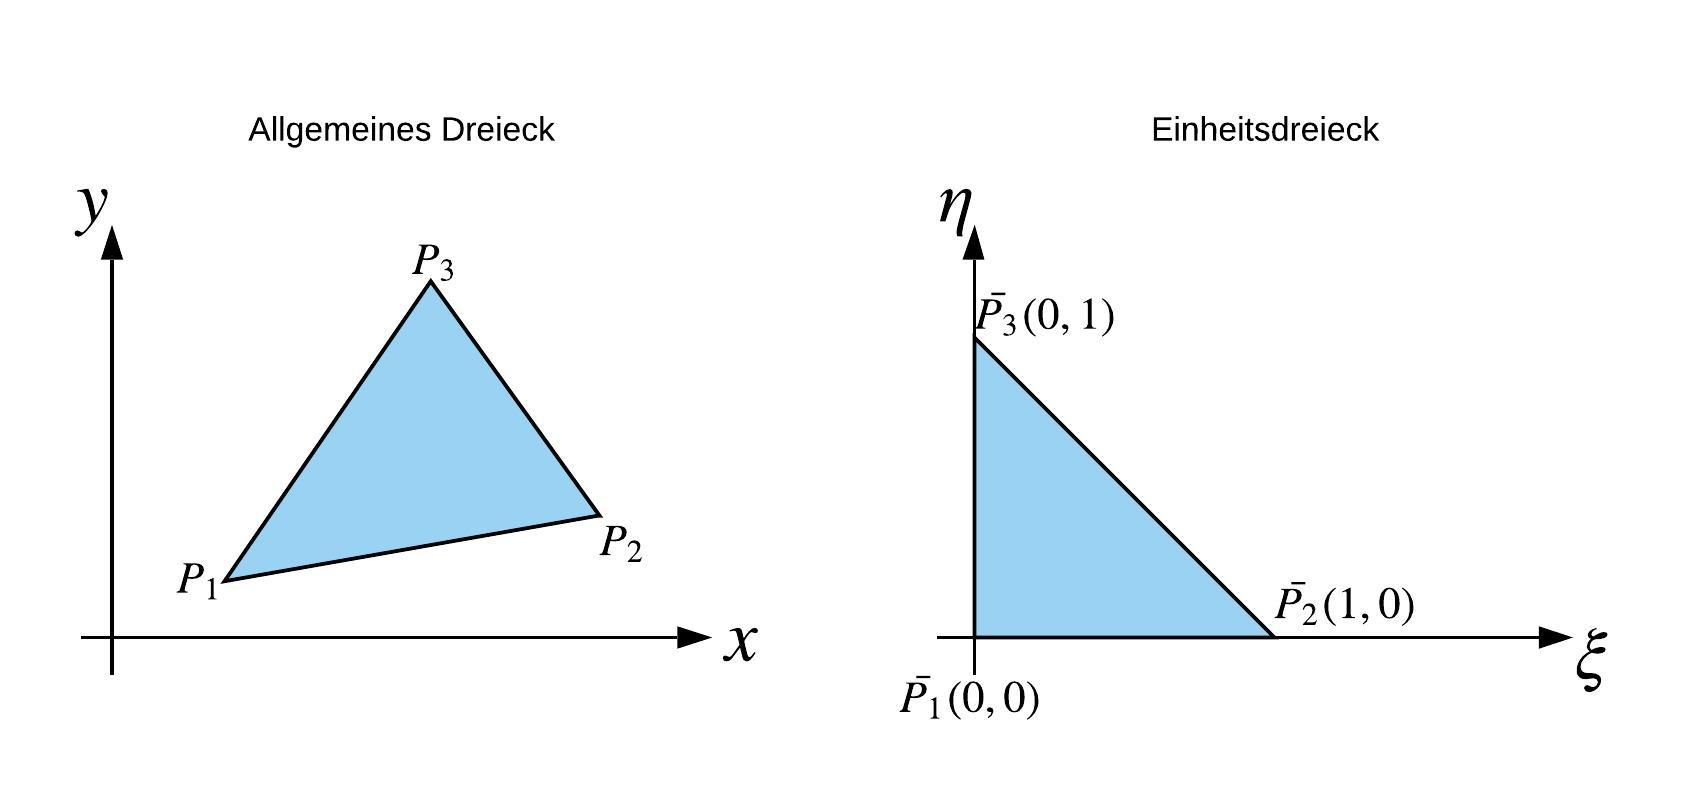
\includegraphics[scale=0.8]{papers/fem/Images/Dreiecke.jpeg}
	\caption{Transformation in ein Einheitsdreieck}
	\label{fig:TransformationEinheitsdreieckBild}
\end{figure}
Die Variablen $\xi$ und $\eta$ werden die neuen Integrationsvariablen. Damit die Berechnung korrekt ist, muss noch die Determinante der Jacobi- Matrix auf der rechten Seite, wie in 
\begin{equation}
			dy \, dy = \det(J) \, d\xi \, d\eta
			\label{fem:newTransformation}
\end{equation}
dargestellt, dazu multipliziert werden wie in \eqref{fem:newTransformation}. Die Jacobi- Matrix
\begin{equation}
J % 
=
\begin{bmatrix}
    \frac{\partial x}{\partial \xi} &  \frac{\partial x}{\partial \eta}     \\
   \frac{\partial y}{\partial \xi}  &  \frac{\partial y}{\partial \eta}     
\end{bmatrix}
= 
\begin{bmatrix}
    x_2 - x_1  &  x_3 -x_1      \\
    y_2 - y_1  &  y_3 - y_1      
\end{bmatrix} \; .
	\label{fem:Jocobi}
\end{equation}
besteht aus den partiellen Ableitungen aus \eqref{fem:linTransformation}. Aus der Transformation \eqref{fem:linTransformation} erhält man 
\begin{equation}
	\det(J) = x_1 \cdot y_2 - 2 \cdot x_1 \cdot y_1 + x_2 \cdot y_1 + x_1\cdot y_3 + x_3 \cdot y_1 - x_2 \cdot y_3 - x_3 \cdot y_2 \; .
	\label{fem:JocobiDetBerechnet}
\end{equation}
Die Jacobi- Determinante \eqref{fem:JocobiDetBerechnet} entspricht der doppelten Fläche des Dreiecks. Die partiellen Ableitungen werden gemäss der Kettenregel zu 
%\begin{equation}
%			\begin{aligned}
%			u_x = u_{\xi} \xi_x + u_{\eta} \eta_x \\
%			u_y = u_{\xi} \xi_y + u_{\eta} \eta_y 
% 			\end{aligned}
%			\label{fem:newKoordinate}
%\end{equation}
\begin{equation}
\begin{split}
	\frac{\partial u}{\partial x} &= \frac{\partial u}{\partial \xi} \, \frac{\partial \xi}{\partial x} + \frac{\partial u}{\partial \eta} \, \frac{\partial \eta}{\partial x} \\
	\frac{\partial u}{\partial y} &= \frac{\partial u}{\partial \xi} \, \frac{\partial \xi}{\partial y} + \frac{\partial u}{\partial \eta} \, \frac{\partial \eta}{\partial y} \; .
	\end{split}
\end{equation}
Auf Grund der linearen Transformation \eqref{fem:linTransformation} ergeben sich nach partieller Differentiation der beiden Beziehungen nach $x$ zunächst

\begin{equation}
			\begin{aligned}
			1  &= (x_2 -x_1) \, \frac{\partial \xi}{\partial x} + (x_3 -x_1) \, \frac{\partial \eta}{\partial x} \\
			0 &= (y_2 -y_1) \, \frac{\partial \xi}{\partial x} + (y_3 -y_1) \, \frac{\partial \eta}{\partial x} \; . \\
			 \end{aligned}
\end{equation}
Nach Auflösung  der beiden Gleichungen nach $\frac{\partial \xi}{\partial x}$ und $\frac{\partial \eta}{\partial x}$ ergibt sich
\begin{equation}
			\frac{\partial \xi}{\partial x} = \frac{y_3 - y_1}{J} \qquad \qquad \frac{\partial \eta}{\partial x} = -\frac{y_2 - y_1}{J} \; .
\end{equation}
Analog nach der partiellen Ableitung nach $y$ erhält man

\begin{equation}
			\frac{\partial \xi}{\partial y} = \frac{x_3 - x_1}{J} \qquad \qquad \frac{\partial \eta}{\partial y} = -\frac{x_2 - x_1}{J} \; .
\end{equation}
Somit vereinfacht sich die Integration über das Einheitsdreieck zu
\begin{equation}
			\int_{\triangle} u \quad dy \, dx = \int_0^1 \int_0^{1 - \xi} \, u \det (J) \, d \eta \, d \xi \; .
\end{equation}

\subsection{Schritt 1: Minimalproblem bilden}

Analog zum Kapitel 7.4.1 muss auch die DGL in der Ebene zuerst in ein äquivalentes Minimalproblem übersetzt werden. Das Minimalproblem für FEM in einer Dimension hatte die Form:

\begin{equation}
			\int_0^1 u \textcolor{red}{'} (x)^2 - \lambda \, u(x)^2 dx \,dy \; .
			\label{fem:Minimal1D}
\end{equation}
Im Unterschied zu den mehrdimensionale Form wird anstatt der einfachen Ableitung der Laplace Operator verwendet, der zugleich zweifache Differenziebarkeit von der Ansatzfunktion $u(x)$ fordert. Zudem wird nicht mehr über eine Strecke integriert sondern über ein Teilgebiet $\Omega_i$:

\begin{equation}
			\int_{\Omega_i} (\textcolor{red}{\nabla} u)^2 - \lambda u^2 dx \, dy \, .
			\label{fem:Minimal2D}
\end{equation}
Der Integrationsterm \eqref{fem:Minimal2D} wird gemäss der Summenregel in zwei Terme zerlegt nämlich 

\begin{equation}
			\int_{\Omega_i} (\nabla u)^2 \, dx \, dy - \lambda \int_{\Omega_i} u^2 dx \, dy \, .
			\label{fem:Minimal2D2Term}
\end{equation}
In einem nächsten Schritt wird das Minimalproblem auf das Element eingeschränkt. Dies wird im folgenden Abschnitt erläutert.

\subsection{Schritt 2: Lösung durch Ansatzfunktionen approximieren}

Die lineare Ansatzfunktion hat wie schon erwähnt die Form
\begin{equation}
u(\xi, \eta) = c_0 + c_1 \xi + c_2 \eta \, .
\label{fem:equationSchwarzLinear}
\end{equation}
Bei näherer Betrachtung fällt jedoch auf, dass in \eqref{fem:equationSchwarzLinear} die Parameter $c_1, c_2$ und $c_3$ von einem Dreieck zu einem anderen Dreieck unterscheiden. Die Ursache liegt insbesondere darin, dass $c_2$ und $c_3$ von den Kanten abhängig sind und die Kanten wiederum können von Dreieck zu Dreieck variieren ($\Omega_i$, $\Omega_j$). Daher ist die lineare Ansatzfunktion 
\begin{equation}
u(\xi, \eta) = \tilde{c_1} + (\tilde{c_2} -\tilde{c_1})\xi + (\tilde{c_3} - \tilde{c_1})\eta
\label{fem:equationLinearMod}
\end{equation}
besser geeignet. In \eqref{fem:equationLinearMod} sind die $c_i^N$ die Funktionswerte in den Ecken und eignen sich somit viel besser, da nur die Eckwerte ohne Einfluss der Kanten berücksichtigt werden wie in Abbildung \ref{fem:Stuestellen} dargestellt. Die Ansatzfunktion \eqref{fem:equationLinearMod} kann somit direkt in die Formel \eqref{fem:Minimal2D} für ein Teilgebiet eingesetzt werden. Ziel ist es, dass die unbekannten Koeffizienten $c_1, c_2 \, $und$ \, c_3$ anhand dieses Verfahrens bestimmt werden. Das zu lösende Integral für ein Teilgebiet hat die Form
\begin{equation}
\int_0^1 \int_0^{1 - \xi} \bigl[ \nabla \, \bigl( \tilde{c_1} + (\tilde{c_2} - \tilde{c_1})\xi + (\tilde{c_3} - \tilde{c_1})\eta \bigr) \, \bigr]^2 - \lambda \bigl[\tilde{c_1} + (\tilde{c_2} - \tilde{c_1})\xi + (\tilde{c_3} -\tilde{c_1})\eta \, \bigr]^2 \, d \eta \, d \xi \; .
\label{fem:FlaecheDreieck}
\end{equation}
\begin{figure}[h]
	\centering
	%
% tikztemplate.tex -- template for standalon tikz images
%
% (c) 2020 Prof Dr Andreas Müller, Hochschule Rapperswil
%
\documentclass[tikz]{standalone}
\usepackage{amsmath}
\usepackage{times}
\usepackage{txfonts}
\usepackage{pgfplots}
\usepackage{csvsimple}
\usetikzlibrary{arrows,intersections,math}
\begin{document}
\def\skala{1}
\begin{tikzpicture}[>=latex,thick,scale=\skala]

\coordinate[] (c1) at (0,0);
\coordinate[] (c2) at (4,0);
\coordinate[] (c3) at (4,2);
\coordinate[] (c4) at (0,2);

 \fill[color=orange] (0,0) -- (4,0) -- (0,2) --cycle;

\draw (c1) node[below]{$c_0^{\triangle_1}$} -- (c2) node[below]{$c_1^{\triangle_1} = c_0^{\triangle_2}$} -- (c4) node[above]{$c_2^{\triangle_1} =c_2^{\triangle_2} $} -- (c1);
\draw (c2) node[below]{$c_1^{\triangle_1} = c_0^{\triangle_2}$} -- (c3) node[above]{$c_1^{\triangle_2}$} -- (c4) node[above]{$c_2^{\triangle_1} =c_2^{\triangle_2}$};

\node at (1.332,0.666) {$\triangle_1$};
\node at (2.664,1.332) {$\triangle_2$};

\end{tikzpicture}
\end{document}


	\caption{Stützstellen der Elemente $\int_{\Omega_1}$ und $\int_{\Omega_2}$ }
	\label{fem:Stuestellen}
\end{figure} 
\begin{figure}[h!]
	\centering
	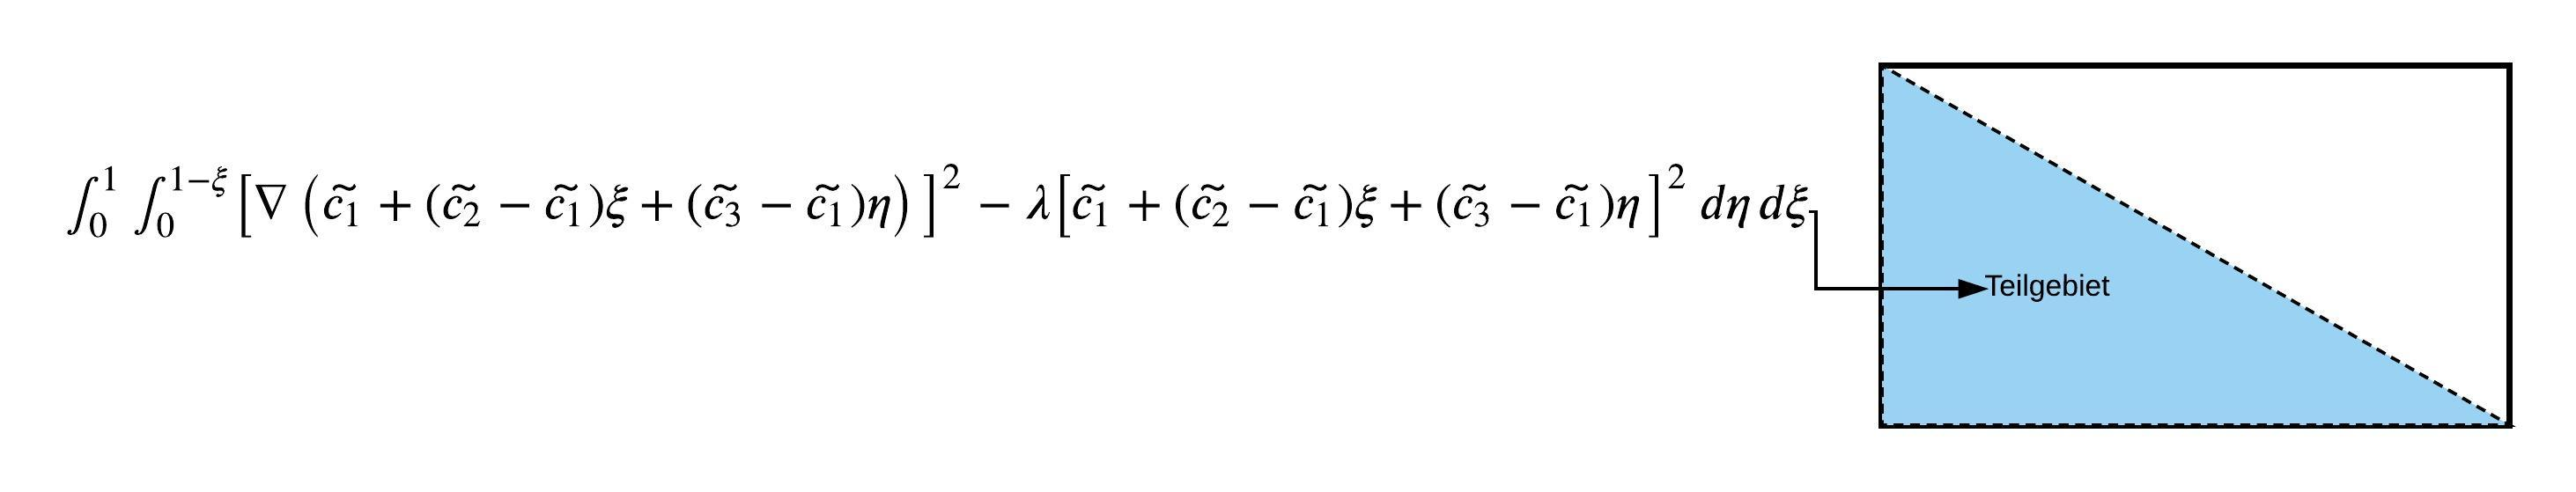
\includegraphics[scale=0.6]{papers/fem/Images/FoTeilgebiet.jpeg}
	\caption{Anwenden der Formel \eqref{fem:FlaecheDreieck} auf jedes Teilgebiet}
	\label{fig:schemNMR_vorlage}
\end{figure}
Allerdings sollte gemäss \eqref{fem:Minimal2D2Term} die Formel \eqref{fem:FlaecheDreieck} aufgeteilt werden in
\begin{equation}
\int_0^1 \int_0^{1 - \xi} \bigl[ \nabla \, \bigl( \tilde{c_1} + (\tilde{c_2} - \tilde{c_1})\xi + (\tilde{c_3} - \tilde{c_1})\eta \bigr) \, \bigr]^2 \, d \eta \, d \xi \; - \; \lambda \int_0^1 \int_0^{1 - \xi} \bigl[\tilde{c_1} + (\tilde{c_2} - \tilde{c_1})\xi + (\tilde{c_3} - \tilde{c_1})\eta \, \bigr]^2 \, d \eta  \, d \xi \, .
\label{fem:IntInt}
\end{equation}

\subsubsection{Berechnung der Integrale}

Im ersten Integralterm von \eqref{fem:IntInt} wird der Gradienten von $u(\xi, \eta)$  quadriert benötigt. Der Gradient von $u(\xi, \eta)$ ist 
\begin{equation}
	\nabla u = 	
	\left[ \begin{array}{r}
	\tilde{c_2} - \tilde{c_1} \\
	\tilde{c_3} - \tilde{c_1} \\
	\end{array}\right] \, .
	\label{fem:equationSchwarzquadratischP22}
\end{equation} 
Der Koeffizient $\tilde{c_1}$ im ersten Integralterm von \eqref{fem:IntInt} verschwindet in \eqref{fem:equationSchwarzquadratischP22}. Der Gradient \ref{fem:equationSchwarzquadratischP22} quadriert ergibt

\begin{equation}
	(\nabla u)^2 = \tilde{c_2}^2 - 2 \tilde{c_1} \tilde{c_2} + \tilde{c_1}^2 + \tilde{c_3}^2 -2 \tilde{c_1}\tilde{c_3} + \tilde{c_1}^2 = 2\tilde{c_1}^2 + \tilde{c_2}^2 + \tilde{c_3}^2 -2\tilde{c_1}\tilde{c_2} -2\tilde{c_1}\tilde{c_3}\, .
	\label{fem:equationSchwarzquadratischQ2}
\end{equation}
Im zweite Integralterm wird 
\begin{multline}
	u(\xi, \eta)^2 = \tilde{c_1}^2 \xi^2  - 2 \tilde{c_1} \tilde{c_2} \xi^2 + \tilde{c_2}^2 \xi^2 + 2 \tilde{c_1}^2 \xi \eta - 2 \tilde{c_1} \tilde{c_2} \xi \eta - 2 \tilde{c_1} \tilde{c_3} \xi \eta + 2 \tilde{c_2} \tilde{c_3} \xi \eta - 2 \tilde{c_1}^2 \xi + \\\ 2 \tilde{c_1} \tilde{c_2} \xi + \tilde{c_1}^2 \eta^2 - 2 \tilde{c_1} \tilde{c_3} \eta^2 + \tilde{c_3}^2 \eta^2 - 2 \tilde{c_1}^2 \eta + 2 \tilde{c_1} \tilde{c_3} \eta + \tilde{c_1}^2 \; .
	\label{fem:vielzuviel}
\end{multline}
Wie in \eqref{fem:vielzuviel} zusehen ist, ist die Berechnung nicht anspruchsvoll, aber aufwändig. Nun ist aber noch die Frage offen wie die Koeffizienten in Matrixform zustande kommen. In folgenden Abschnitt wird dies anhand eines Beispiels beschrieben.

\subsubsection{Matrixform der Integrale
\label{fem:section:GL}}

Da die Ansatzfunktion \eqref{fem:equationLinearMod} zwar unabhängig von den Kanten ist, aber die Berechnung des Quadrates von $u$ \eqref{fem:vielzuviel} unübersichtlich, wird in diesem Beispiel in diesem Abschnitt die lineare Ansatzfunktion \eqref{fem:equationSchwarzLinear} verwendet. Somit ist
\begin{equation}
	\nabla u = 	
	\left[ \begin{array}{r}
	c_1 \\
	c_2 \\
	\end{array}\right] \; \Longrightarrow \; (\nabla u)^2 = c_1^2 + c_2^2
	\label{fem:equationSchwarzquadratischPP}
\end{equation}  
und 
\begin{equation}
 	u^2 = \textcolor{cyan}{c_0^2} + \textcolor{blue}{c_1^2 x^2} + \textcolor{red}{c_2^2 y^2} + \textcolor{green}{2 c_0 c_1 x} + \textcolor{orange}{2 c_0 c_2 y} +\textcolor{purple}{ 2 c_1 c_2 xy} \, .
	\label{fem:equationSchwarzquadratischQQQ}
\end{equation}  
Bekannt ist nun, wie die Integrale für die einzelne Teilgebiete aussehen. Um eine Matrixnotation der Koeffizienten $c_i$ zu erhalten, um dann ein Gleichungssystem für deren Berechnung aufzubauen, werden die Koeffizienten in Vektorform
\begin{equation}
	\begin{bmatrix}
	c_0^{(\triangle_i)}  \\
	c_1^{(\triangle_i)} \\
	c_2^{(\triangle_i)}
	\end{bmatrix}
	\label{fem:VektorAlg}
\end{equation}
aufgeschrieben. In \eqref{fem:VektorAlg} ist die Vektornotation der Koeffizienten von \eqref{fem:equationSchwarzLinear}. Nun wird der Integraltem
\begin{equation}
			\underbrace{ \int_{\Omega_i} (\nabla u)^2 d\xi \, d\eta}_{\text{1. Term}} \, -  \, \underbrace{\lambda \int_{\Omega_i} u^2 d\xi \,d\eta}_{\text{2. Term}}
			\label{fem:Minimal2TermLinAlg}
\end{equation}
eines Teilgebietes in die lineare Notation
\begin{equation}
			\underbrace{ c^t Ac}_{\text{1. Term}} \, - \, \underbrace{\lambda c^t Bc}_{\text{2. Term}}
			\label{fem:Minimal2LinAlg}
\end{equation}
gebracht. Gemäss \eqref{fem:Minimal2TermLinAlg} sind Quadrate der Koeffizienten $c_i$ gefordert. Um nun quadratische Koeffizienten in der Matrixschreibweise zu erhalten wird dies wie folgt notiert:
\begin{equation}
\begin{bmatrix}
c_0^{(\triangle_i)} &  c_1^{(\triangle_i)} &  c_2^{(\triangle_i)}  
\end{bmatrix}
\begin{bmatrix}
\ddots & \cdots &  \cdots    \\
\vdots & \ddots &   \\
\vdots &  & \ddots
\end{bmatrix}
\begin{bmatrix}
c_0^{(\triangle_i)}  \\
c_1^{(\triangle_i)} \\
c_2^{(\triangle_i)}
\end{bmatrix}
+
\lambda
\begin{bmatrix}
c_0^{(\triangle_i)} &  c_1^{(\triangle_i)} &  c_2^{(\triangle_i)}    \\   
\end{bmatrix}
\begin{bmatrix}
\ddots & \cdots &  \cdots    \\
\vdots & \ddots &   \\
\vdots &  & \ddots
\end{bmatrix}
\begin{bmatrix}
c_0^{(\triangle_i)}  \\
c_1^{(\triangle_i)} \\
c_2^{(\triangle_i)}
\end{bmatrix} \; .
	\label{fem:MatrixKoeffizient}
\end{equation}
Dies ist auch die Begründung warum Formel \eqref{fem:Minimal2LinAlg} verwendet wird.
%Für jedes Flächenelement gilt die Gleichung \ref{fem:MinimalproblemElement}. Nun müssen alle diese Elemente in eine Matrix umgeschrieben werden die sich wie folgt zusammensetzen lässt.
Die Matrix $A$ wird gebildet durch die Teilmatrizen eines jeden Teilgebietes. Die Teilmatrix eines Teilgebiet besteht  aus dem Integral des 1. Terms von \eqref{fem:Minimal2TermLinAlg} 

\begin{equation}
			\int_0^1 \int_0^{1 - \xi} \left( \begin{array}{c} c_1 \\ c_2 \\	
\end{array} \right)^2 d\eta \, d\xi
			\label{fem:Minimal2LinAlgA}
\end{equation}
was dann zu der entsrechenden Teilmatrix
\begin{equation}
	A_{\triangle_i} = \left( \begin{array}{cc}
	\int_{\Omega_i} 1 d\eta \, d\xi & 0  \\ 
	0 & \int_{\Omega_i} 1 d\eta \, d\xi  \\
	\end{array}\right)
	\label{fem:TeilmatrixA}
\end{equation}
Hier gibt es ein Problem. Der Koeffizient $c_0$ ist hier nicht berücksichtigt. Es wird eine Matrix $A_{\triangle_i}$ derart benötigt so, dass
 \begin{equation}
	\int_{\triangle_i} (\nabla u)^2 d\xi d\eta = c^tAc
	\label{fem:KeiAhnig}
\end{equation}
Daher wird die Matrix
\begin{equation}
	A_{\triangle_i} = \left( \begin{array}{ccc}
	0 & 0 & 0 \\
	0 &  \int_{\Omega_i} 1 d\eta \, d\xi & 0  \\ 
	0 & 0 & \int_{\Omega_i} 1 d\eta \, d\xi  \\
	\end{array}\right)
	\label{fem:TeilmatrixA}
\end{equation}
mit Nullen entsprechend angepasst. Die Teilmatrix ausgerechnet ergibt
\begin{equation}
	A_{\triangle_i} = \left( \begin{array}{ccc}
	0 & 0 & 0 \\
	0 & \frac{1}{2} & 0  \\ 
	0 & 0 &  \frac{1}{2}\\
	\end{array}\right)
\end{equation}
und wird dann in die grosse Matrix $A$ eingefügt. Wie genau die Teilmatrizen $A_{\triangle_i}$ in eine gesamte Matrix A zusammengesetzt werden, wird weiter unten am Beispiel der Matrix B erläutert. 

%\begin{equation}
% A = \begin{pmatrix} 0 & 0 & \hdotsfor{4} & 0 \\
%	0 & \textcolor{green}{ c_2^2 \int_{\Omega} 1 dx \, dy }& \vdots & 0 & \vdots &\vdots  & \vdots \\
%	\vdots & \vdots & \textcolor{green}{c_3^2 \int_{\Omega} 1 dx \, dy }& 0 & \vdots  & & \\
%	\vdots & \vdots & 0 & \ddots & \textcolor{red}{ c_2^2 \int_{\Omega} 1 dx \, dy }& & \vdots \\
%	\vdots & \vdots & 0 & 0 & 0 & \textcolor{red}{c_3^2 \int_{\Omega} 1 dx \, dy} & \\
%	0 & \hdotsfor{2} & 0 &  & & &  \ddots  \\
%	\end{pmatrix}
%	\label{fem:MatrixA}
%\end{equation}
%\begin{equation}
% A =	\begin{pmatrix}
%	\textcolor{green}{A_{\triangle_1} }& 0 & \cdots & \cdots & 0 \\
%	0 & \ddots & \vdots & 0 & \vdots \\
%	\vdots & \vdots & \ddots & 0 & \vdots \\
%	\vdots & \vdots & 0 & \textcolor{red}{A_{\triangle_i}} & \vdots \\
%	0 & \cdots & \cdots & 0 &  \ddots \\
%	\end{pmatrix}
%\end{equation}
%Die Koeffizienten werden ausserhalb der Matrix $A$ geschrieben, so dass diese in einem weiteren Schritt berechnet werden können durch ein Gleichungssystem.
%\begin{equation}
%\begin{bmatrix}
%c_1^0 &  c_1^1 &  c_1^2  
%\end{bmatrix}
%\begin{bmatrix}
%\ddots & \cdots &  \cdots    \\
%\vdots & \ddots &   \\
%\vdots &  & \ddots
%\end{bmatrix}
%\begin{bmatrix}
%c_1^0  \\
%c_1^1 \\
%c_1^2
%\end{bmatrix}
%\end{equation}
Die Matrix $A$ ist nun bekannt. Es fehlt jedoch noch die Matrix $B$, um das Gleichungssystem zu komplettieren. Die Matrix $B$ wird nun wie folgt definiert. Um die folgende Form in \eqref{fem:Minimal2LinAlgB} zu erhalten muss lediglich der zweite Term von \eqref{fem:Minimal2TermLinAlg} für die einzelnen Koeffizienten berechnet werden, was dann den folgenden Ausdruck

\begin{equation}
			\int_0^1 \int_0^{1 - \xi}  \textcolor{cyan}{c_0^2} + \textcolor{blue}{c_1^2 x^2} + \textcolor{red}{c_2^2 y^2} + \textcolor{green}{2 c_0 c_1 x} + \textcolor{orange}{2 c_0 c_2 y} +\textcolor{purple}{ 2 c_1 c_2 xy} \,  d\eta \, d \xi
			\label{fem:Minimal2LinAlgB}
\end{equation}
ergibt. Nun soll dies wieder in die Matrix- Schreibweise übertragen werden was dann einer Teilmatrix

\begin{equation}
 B_{\triangle_i} = \left( \begin{array}{ccc}
	\textcolor{cyan}{- \lambda \int_{\Omega_i} 1} &  \textcolor{green}{- \lambda \int_{\Omega_i} x} & \textcolor{orange}{- \lambda \int_{\Omega_i} y}  \\
	\textcolor{green}{- \lambda \int_{\Omega_i}x} & \textcolor{blue}{- \lambda \int_{\Omega_i} x^2} &  \textcolor{purple}{- \lambda \int_{\Omega_i} xy} \\
	\textcolor{orange}{- \lambda \int_{\Omega_i} y} & \textcolor{purple}{- \lambda \int_{\Omega_i} xy} & \textcolor{red}{ - \lambda \int_{\Omega_i} y^2} \\
	\end{array}\right)
	\label{fem:MatrixB}
\end{equation}
eines Dreickes entsprich und ausgerechnet
\begin{equation}
 B_{\triangle_i} = - \lambda \left( \begin{array}{ccc}
	\textcolor{cyan}{ \frac{1}{2}} &  \textcolor{green}{ \frac{1}{6}}& \textcolor{orange}{\frac{1}{3}}  \\
	\textcolor{green}{\frac{1}{6}} & \textcolor{blue}{\frac{1}{12}} &  \textcolor{purple}{ \frac{1}{24}} \\
	\textcolor{orange}{\frac{1}{3}} & \textcolor{purple}{\frac{1}{24}} & \textcolor{red}{ \frac{1}{12}} \\
	\end{array}\right) 
	\label{fem:MatrixB}
\end{equation}
ergibt.

\subsubsection{Zusammensetzten der Teilmatrizen $A$ und $B$}
Anhand eines Beispieles soll gezeigt werden wie sich die $B$ Matrix aus den Teilmatrizen $B_{\triangle_i}$ zusammenstellt. Als Beispiel dient eine Approximation mit den beiden Dreiecken $\textcolor{red}{\triangle_1}$ und $\textcolor{blue}{\triangle_2}$
\begin{figure}[h]
	\centering
	%
% dreiecke.tex -- Dreiecke Kombination der Matrizen
%
% (c) 2020 Prof Dr Andreas Müller, Hochschule Rapperswil
%
\documentclass[tikz]{standalone}
\usepackage{amsmath}
\usepackage{times}
\usepackage{txfonts}
\usepackage{pgfplots}
\usepackage{csvsimple}
\usetikzlibrary{arrows,intersections,math}
\begin{document}
\def\skala{1}
\begin{tikzpicture}[>=latex,thick,scale=\skala]

\definecolor{farbe1}{rgb}{0.8,0,0}
\definecolor{farbe2}{rgb}{0,0,1}

\coordinate (C1) at (0,0);
\coordinate (C2) at (2,0);
\coordinate (C3) at (4,1);
\coordinate (C4) at (1,2);

\coordinate (S1) at (1,0.6666);
\coordinate (S2) at (2.333,1);

\fill[color=farbe1!20] (C1) -- (C2) -- (C4) -- cycle;
\fill[color=farbe2!20] (C2) -- (C3) -- (C4) -- cycle;

\draw[color=farbe1] (C1)--(C2)--(C4)--cycle;
\draw[color=farbe2] (C2)--(C3)--(C4)--cycle;

\node[color=farbe1] at (S1) {$\triangle_1$};
\node[color=farbe2] at (S2) {$\triangle_2$};

\fill (C1) circle[radius=0.08];
\fill (C2) circle[radius=0.08];
\fill (C3) circle[radius=0.08];
\fill (C4) circle[radius=0.08];

\node at (C1) [below left] {$c_1$};
\node at (C2) [below] {$c_2$};
\node at (C3) [right] {$c_3$};
\node at (C4) [above] {$c_4$};

\end{tikzpicture}
\end{document}


	\caption{Zwei Dreiecke mit gemeinsamen Stützstellen $c_2$ und $c_4$ }
\end{figure}
Das Dreieckgebiet $\textcolor{red}{\triangle_1}$ hat

\begin{equation}
\int_{\triangle_1} u^2 d\eta \; d\xi = \begin{bmatrix}
c_1 &  c_2 &  c_4  
\end{bmatrix}
\begin{bmatrix}
 & &      \\
 & B_1 &   \\
 &  & 
\end{bmatrix}
\begin{bmatrix}
c_1  \\
c_2 \\
c_4
\end{bmatrix}
\end{equation}
als Matrixform und das Gebiet $\textcolor{blue}{\triangle_2}$

\begin{equation}
\int_{\triangle_2} u^2 d\eta \; d\xi = \begin{bmatrix}
c_2 &  c_3 &  c_4  
\end{bmatrix}
\begin{bmatrix}
 & &      \\
 & B_2 &   \\
 &  & 
\end{bmatrix}
\begin{bmatrix}
c_2  \\
c_3 \\
c_4
\end{bmatrix} \; .
\end{equation}
Beide Gebiete zusammen entsprechen 

\begin{equation}
\int_{\triangle_1 und \triangle_2} u^2 d\eta \; d\xi = \int_{\triangle_1} u^2 d\eta \; d\xi + \int_{\triangle_2} u^2 d\eta \; d\xi = c_{\triangle_1}^t B_1 c_{\triangle_1} + c_{\triangle_2}^t B_2 c_{\triangle_2} \; .
\end{equation}
Die Koeffizienten von $\textcolor{red}{\triangle_1}$ sind

\begin{equation}
\int_{\triangle_1} \underbrace{c_1^2}_{\textcolor{red}{\frac{1}{2}}} + \underbrace{c_2^2 \; \xi^2}_{\textcolor{red}{\frac{1}{12}}} + \underbrace{c_4^2 \; \eta^2}_{\textcolor{red}{\frac{1}{12}}} + \underbrace{2 c_1 c_2\; \xi}_{\textcolor{red}{\frac{1}{6}}} + \underbrace{2 c_1 c_4 \; \eta}_{\textcolor{red}{\frac{1}{3}}} + \underbrace{2 c_2 c_4}_{\textcolor{red}{\frac{1}{24}}} d\eta \; d\xi
\label{fem:roteKoeffizienten}
\end{equation}
und von $\textcolor{blue}{\triangle_2}$ 
\begin{equation}
\int_{\triangle_2} \underbrace{c_2^2}_{\textcolor{blue}{\frac{1}{2}}} + \underbrace{c_3^2 \; \xi^2}_{\textcolor{blue}{\frac{1}{12}}} + \underbrace{c_4^2 \; \eta^2}_{\textcolor{blue}{\frac{1}{12}}} + \underbrace{2 c_2 c_3 \; \xi}_{\textcolor{blue}{\frac{1}{6}}} + \underbrace{2 c_2 c_4 \; \eta}_{\textcolor{blue}{\frac{1}{3}}} + \underbrace{2 c_3 c_4}_{\textcolor{blue}{\frac{1}{24}}} d\eta \; d\xi \; .
\label{fem:blaueKoeffizienten}
\end{equation}

Bevor die roten und blauen Koeffizienten von \eqref{fem:roteKoeffizienten} und \eqref{fem:blaueKoeffizienten} der jeweiligen Gebiete zusammengesetzt werden können, gemäss der Abbildung \ref{fem:MatrixBKomplett}, müssen zwei Punkte berücksichtigt werden:
\begin{itemize}
	\item Jeder Koeffizient muss nach \eqref{fem:newTransformation} mit dem dazugehörigen Jacobi- Determinante \eqref{fem:JocobiDetBerechnet} des eignen Dreiecks multipliziert werden. 
	\item Es müssen die $\tilde{c}$- Variablen verwendet werden. Die Umrechnung ist in  \ref{fem:section:loesungTrans} beschrieben.
\end{itemize}
Sind die beiden Schritte durchgeführt, können die Koeffizienten gemäss der Abbildung \ref{fem:MatrixBKomplett} die Matrix $B$ gebildet werden.
\begin{figure}[h]
	\centering
	%
% matrizen.tex -- matrizen
%
% (c) 2020 Prof Dr Andreas Müller, Hochschule Rapperswil
%
\documentclass[tikz]{standalone}
\usepackage{amsmath}
\usepackage{times}
\usepackage{txfonts}
\usepackage{pgfplots}
\usepackage{csvsimple}
\usetikzlibrary{arrows,intersections,math}
\begin{document}
\def\skala{1}
\begin{tikzpicture}[>=latex,thick,scale=\skala]

\definecolor{farbe1}{rgb}{1,0,0}
\definecolor{farbe2}{rgb}{0,0,1}

\def\xstep{0.82}
\def\ystep{0.595}
\def\xorg{-0.43}
\def\yorg{-0.625}

\begin{scope}[xshift=-3cm,yshift=3cm]

\foreach \x in {0,1,2}{
	\foreach \y in {0,1,2}{
		\fill[color=farbe1!20]
			({\xorg+(\x-0.3)*\xstep},{\yorg+(\y-0.4)*\ystep})
			rectangle
			({\xorg+(\x+0.3)*\xstep},{\yorg+(\y+0.4)*\ystep});
	}
}


\node at (0,0) {$\displaystyle
\renewcommand\arraystretch{1.4}
B_1 = \begin{pmatrix}
\;\;\frac12\;\; & \frac16    & \;\;\frac13  \;\; \\
\frac16 & \frac1{12} & \frac1{24}\\
\frac13 & \frac1{24} & \frac1{12}
\end{pmatrix}
$};

\end{scope}

\begin{scope}[xshift=3cm,yshift=3cm]

\foreach \x in {0,1,2}{
	\foreach \y in {0,1,2}{
		\fill[color=farbe2!20]
			({\xorg+(\x-0.3)*\xstep},{\yorg+(\y-0.4)*\ystep})
			rectangle
			({\xorg+(\x+0.3)*\xstep},{\yorg+(\y+0.4)*\ystep});
	}
}

\node at (0,0) {$\displaystyle
\renewcommand\arraystretch{1.4}
B_2 = \begin{pmatrix}
\;\;\frac12\;\; & \frac16    & \;\;\frac13\;\;   \\
\frac16 & \frac1{12} & \frac1{24}\\
\frac13 & \frac1{24} & \frac1{12}
\end{pmatrix}
$};

\end{scope}

\def\xstep{1.35}
\def\ystep{0.593}
\def\xorg{-1.71}
\def\yorg{-0.91}

\foreach \x in {0,1,3}{
	\foreach \y in {0,2,3}{
		\fill[color=farbe1!20]
			({\xorg+(\x-0.4)*\xstep},{\yorg+(\y-0.4)*\ystep})
			rectangle
			({\xorg+(\x+0.4)*\xstep},{\yorg+(\y+0.4)*\ystep});
	}
}

\foreach \x in {1,2,3}{
	\foreach \y in {0,1,2}{
		\fill[color=farbe2!20]
			({\xorg+(\x-0.4)*\xstep},{\yorg+(\y-0.4)*\ystep})
			rectangle
			({\xorg+(\x+0.4)*\xstep},{\yorg+(\y+0.4)*\ystep});
	}
}

\foreach \x in {1,3}{
	\foreach \y in {0,2}{
		\fill[color=farbe1!20]
			({\xorg+(\x-0.4)*\xstep},{\yorg+(\y+0.4)*\ystep})
			--
			({\xorg+(\x-0.4)*\xstep},{\yorg+(\y-0.4)*\ystep})
			--
			({\xorg+(\x+0.4)*\xstep},{\yorg+(\y+0.4)*\ystep})
			--cycle;
	}
}


\node at (0,0) {$\displaystyle
\renewcommand\arraystretch{1.4}
B = \begin{pmatrix}
\frac12 & \frac16              &  \phantom{\frac1{24}+\frac1{12}}          & \frac13                \\
\frac16 & \frac1{12} + \frac12 & \frac16     & \frac1{24}+\frac13     \\
 \phantom{\frac1{24}+\frac1{12}}             & \frac16              & \frac1{12}  & \frac1{24}             \\
\frac13 & \frac1{24} + \frac13 & \frac1{24}  & \frac1{12} + \frac1{12}
\end{pmatrix}
$};

\draw[->,line width=1.4pt] (-1.7,1.9) -- (-0.8,1.3);
\draw[->,line width=1.4pt] (2.3,1.9) -- (1.4,1.3);

\end{tikzpicture}
\end{document}


	\caption{Matrix $B$ zusammenstellen }
	\label{fem:MatrixBKomplett}
\end{figure}
Das Vorgehen für die Matrix $A$ ist genau gleich. 
Wie sieht die Matrix aus wenn mit mehr Dreiecken approximiert wird? Bei einem $5 \times 5$ Gitter mit 36 Variablen hätte die Matrix $B$ die Form wie in Abbildung \ref{fem:MatrixBGross} .

\begin{figure}[h]
	\centering
	%
% gross.tex -- groesseres Gitter
%
% (c) 2020 Prof Dr Andreas Müller, Hochschule Rapperswil
%
\documentclass[tikz]{standalone}
\usepackage{amsmath}
\usepackage{times}
\usepackage{txfonts}
\usepackage{pgfplots}
\usepackage{csvsimple}
\usetikzlibrary{arrows,intersections,math}
\begin{document}
\def\skala{1}
\begin{tikzpicture}[>=latex,thick,scale=\skala]

\definecolor{farbe1}{rgb}{0.8,0,0}
\definecolor{farbe2}{rgb}{0,0,1}

\foreach \x in {0,...,4}{
	\foreach \y in {0,...,4}{
		\fill[color=farbe1!20] (\x,\y) -- ({\x+1},{\y+1}) -- (\x,{\y+1}) --cycle;
		\fill[color=farbe2!20] (\x,\y) -- ({\x+1},\y) -- ({\x+1},{\y+1}) --cycle;
	}
}
\foreach \x in {0,...,5}{
	\draw (\x,0) -- (\x,5);
}
\foreach \y in {0,...,5}{
	\draw (0,\y) -- (5,\y);
}
\foreach \x in {0,...,4}{
	\foreach \y in {0,...,4}{
		\draw (\x,\y) -- ({\x+1},{\y+1});
	}
}

\foreach \x in {0,...,5}{
	\foreach \y in {0,...,5}{
		\fill (\x,\y) circle[radius=0.08];
	}
}

\foreach \x in {0,...,5}{
	\node at (\x,0) [above left] {$\x$};
}
\foreach \x in {6,...,11}{
	\node at ({\x-6},1) [above left] {$\x$};
}
\foreach \x in {12,...,17}{
	\node at ({\x-12},2) [above left] {$\x$};
}
\foreach \x in {18,...,23}{
	\node at ({\x-18},3) [above left] {$\x$};
}
\foreach \x in {24,...,29}{
	\node at ({\x-24},4) [above left] {$\x$};
}
\foreach \x in {30,...,35}{
	\node at ({\x-30},5) [above left] {$\x$};
}

\def\xstep{0.145}
\def\ystep{-0.145}

\def\quadrat#1#2#3{
	\fill[color=#3,opacity=0.2]
		({({#1}-0.5)*\xstep},{({#2}-0.5)*\ystep})
		rectangle
		({({#1}+0.5)*\xstep},{({#2}+0.5)*\ystep});
}

\def\oberesdreieck#1{
	\quadrat{#1}{#1}{farbe1}
	\quadrat{#1+6}{#1}{farbe1}
	\quadrat{#1+7}{#1}{farbe1}
	\quadrat{#1}{#1+6}{farbe1}
	\quadrat{#1+6}{#1+6}{farbe1}
	\quadrat{#1+7}{#1+6}{farbe1}
	\quadrat{#1}{#1+7}{farbe1}
	\quadrat{#1+6}{#1+7}{farbe1}
	\quadrat{#1+7}{#1+7}{farbe1}
}

\def\unteresdreieck#1{
	\quadrat{#1}{#1}{farbe2}
	\quadrat{#1+1}{#1}{farbe2}
	\quadrat{#1+7}{#1}{farbe2}
	\quadrat{#1}{#1+1}{farbe2}
	\quadrat{#1+1}{#1+1}{farbe2}
	\quadrat{#1+7}{#1+1}{farbe2}
	\quadrat{#1}{#1+7}{farbe2}
	\quadrat{#1+1}{#1+7}{farbe2}
	\quadrat{#1+7}{#1+7}{farbe2}
}

\begin{scope}[xshift=7cm,yshift=5cm]

\foreach \i in {0,...,4}{
	\foreach \j in {0,...,4}{
		\oberesdreieck{\i+6*\j}
		\unteresdreieck{\i+6*\j}
	}
}

\end{scope}

\node at (9.2,2.45) {$\displaystyle 
B=\begin{pmatrix}
\hspace*{5.5cm}\\
\\
\\
\\
\\
\\
\\
\\
\\
\\
\\
\\
\\
\end{pmatrix}$};

\end{tikzpicture}
\end{document}


	\caption{$5 \times 5$}
	\label{fem:MatrixBGross}
\end{figure}


\subsection{Schritt 3: Minimalprinizip anwenden auf Approximation}

Nun folgt der nächste Schritt nämlich das Minimieren des quadratischen Ausdrucks
\begin{equation}
	c^t Ac - c^t \lambda Bc \; .
	\label{fem:cAcbc}
\end{equation}
Der Ausdruck \eqref{fem:cAcbc} nach den Koeffizienten $c_k$ abgeleitet ergibt den  für 1. Term
\begin{equation}
	\nabla c^t Ac = 2Ac
\end{equation}
und für den 2. Term den Ausdruck

\begin{equation}
	\nabla c^t \lambda Bc = 2\lambda Bc \; .
\end{equation}
Diese Ableitungen erscheinen nicht gerade ersichtlich insbesondere der Faktor 2.
Das Ableiten im  eindimensionalen Raum ergibt nach der klassichen Analysis

\begin{equation}
	\frac{d}{dx} ax^2 = 2ax \; .
\end{equation}
%Um die Ableitung in einem n-Dimensionalen, quadratischen Matrix vorzunehmen muss diese erst in einen Summennotation umgeschrieben werden wie folgt
Die Ableitung von $x^tAx, x \in \mathbb{R}^n $ nach $x_n$ ergibt nach der Produktregel
\begin{equation}
	\frac{\partial}{\partial x_u} \; x^tAx = \sum_{i,j} \frac{\partial x_i}{\partial x_n} a_{ij} x_j + \sum_{i,j} x_i a_{ij} \frac{\partial x_j}{\partial x_n} \; .
\end{equation}
Dies kann vereinfacht werden anhand der Kürzungs- Berechnung

\begin{equation}
	\sum_{j} a_{nj} x_j + \sum_{i,j} x_i a_{in} = \sum_{j} a_{nj} x_j + \sum_{\textcolor{red}{\not{j}} i} a_{n \textcolor{red}{\not{j}} i} x_{\textcolor{red}{\not{j}} i} = 2(Ax)_n \; .
\end{equation}

\subsection{Schritt 4: Gleichungssystem aufstellen}
Nun kann das Gleichungssystem aufgestellt werden:
\begin{equation}
	2Ac - 2\lambda Bc = 0 \Rightarrow (A-\lambda B)c = 0 \; .
	\label{fem:GLLang}
\end{equation}
Durch das Umschreiben der Gleichung \eqref{fem:GLLang} in 

\begin{equation}
		B^{-1}Ac = \lambda c
 \end{equation}
 ist ersichtlich, dass es sich um ein Eigenwertproblem für die Matrix $B^{-1}A$ handelt. % Dieses kann z.B. durch das Jacobi Verfahren, beschrieben im Kapitel 6.4 gelöst werden.
 Dieses kann z.B. mit dem Francis- Algorithmus, beschrieben im Kapitel 22, gelöst werden.
\subsection{Andere lineare Ansatzfunktionen
\label{fem:subsection:Ansatzfunktionen}}

Neben dem durchgerechneten Beispiel des Einheitsdreiecks kann auch eine andere Gebietsform verwendet werden. Die Funktion

\begin{equation}
	u(x,y) = c_1 + c_2 x + c_3 y + c_4 xy
\end{equation} 
gilt für den linearen Ansatz eines Parallelogramms.

\subsubsection{Quadratischer Ansatz
\label{fem:subsection:bonorum}}

Der Vorteil des quadratischen Ansatzes liegt darin, dass die Freiheitsgeraden erhöht werden. Somit kann unter umständen eine bessere Approximation erreicht werden.
Zu beachten ist allerdings, dass diese die Matrix enorm aufblasen bzw. vergrössern und dann mehr Ressourcen in Anspruch nehmen, um die Matrix bzw. die Eigen werte zu berechnen.

In dem Ausdruck
\begin{align}
	u(x,y) &= c_1 + c_2 x + c_3 y + c_4 x^2 + c_5 xy + c_6 y^2 \label{fem:equationSchwarzquadratischD} \\ 
\end{align}	
ist der Ansatz für das Einheitsdreieck gegeben. Und in der Formel
\begin{align}
u(x,y) &= c_1 + c_2 x + c_3 y + c_4 x^2 + c_5 xy + c_6 y^2 + c_7 x^2y + c_8 xy^2 \label{fem:equationSchwarzquadratischP}
\end{align}
der quadratische Ansatz für ein Einheitsparallelogramm.




